\chapter{Einleitung}
%%Einleitung
%Thema
%Erläuterung des Problems
%Aufgabe/Ziel

In dieser Seminararbeit soll eine mobile Pumpe zur Beförderung von flüssigem Beton, wie sie im Baubereich eingesetzt wird, aus regelungstechnischer Sicht untersucht werden.

%Grafik
\begin{figure}[h!]
\centering
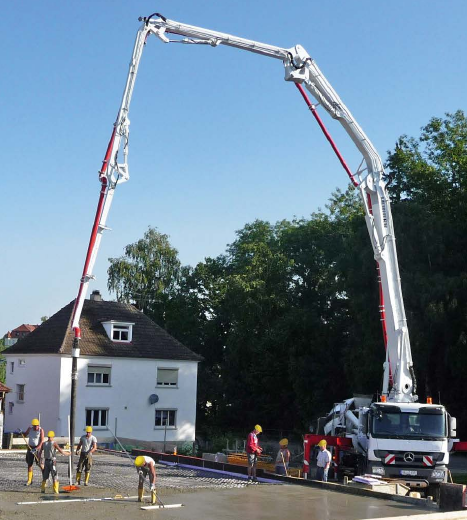
\includegraphics[scale=0.6]{betonpumpe.png}
\caption[]{Mobile Betonpumpe mit ausgefahrenem Ausleger, Quelle: Liebherr}
\end{figure}

In der oberen Darstellung ist eine mobile Betonpumpe bestehend aus Ausleger und LKW-Chassis zusehen. Der Ausleger besteht aus fünf Teilen und lässt sich über Hydraulikzylinder und eine Umlenkkinematik in verschiedene Stellungen fahren. Am Chassis ist außerdem ein  Abstützsystem angebracht, welches Kräfte, die vom Ausleger ausgehen, ableitet. Es bietet darüber hinaus auch in unebenem Gelände Halt.\\

\begin{table}[h!]
\centering
\begin{tabular}{c|c|c}
\rule[-1ex]{0pt}{2.5ex} Armsegment & Masse/kg & Länge/m \\ 
\hline \rule[-1ex]{0pt}{2.5ex} 1 & 2250 & 9 \\ 
\rule[-1ex]{0pt}{2.5ex} 2 & 1700 & 8 \\ 
\rule[-1ex]{0pt}{2.5ex} 3 & 1350 & 7 \\ 
\rule[-1ex]{0pt}{2.5ex} 4 & 900 & 7 \\ 
\rule[-1ex]{0pt}{2.5ex} 5 & 480 & 6 \\ 
\end{tabular} 
\caption{Beispielwerte, welche aus gegebener Gesamtmasse und Gesamtlänge ermittelt wurden}
\label{tab:WertePumpe}
\end{table}

Tabelle \ref{tab:WertePumpe} enthält Werte, welche aus der Gesamtmasse und Gesamtlänge abgeschätzt wurden.

\section{Probleme}
Aufgrund der Leichtbauweise und dem damit verbundenen elastischem Verhalten des Materials kommt es durch den diskontinuierlichen Pumpvorgang zum Schwingen des Auslegers. Das Problem kann mit einer aktiven oder passiven Schwingungsdämpfung eingeschränkt werden. Die aktive Schwingungsdämpfung stellt einen geschlossenen Regelkreis dar. Die Biegung kann dabei bspw. über Dehnungsmessstreifen erfasst werden und über ein Stellsignal auf die Hydraulikzylinder korrigiert werden. Bei der passiven Schwingungsdämpfung wird versucht, über konstruktive Maßnahmen die Schwingung zu dämpfen. Das kann z.B. durch den Einsatz von bestimmten Materialien erreicht werden. Ein anderer Ansatz ist die Verwendung von passiven Vibrations-Absorbern. 

\section{Aufgabe}
In dieser Arbeit soll lediglich die aktive Schwingungsdämpfung betrachtet werden. Es soll eine Regelung entworfen werden und zusätzlich eine Steuerung um den Aktor in verschiedene Stellungen überführen zu können. \\
Als erstes soll ein Modell für, welches die Dynamik des Auslegers abbildet, gefunden werden. Dann soll unter Verwendung der Programmiersprache Python mit Hilfe einer Simulation der Steuerungs- und Regelungsentwurf erfolgen. Die Steuerung sollte dafür sorgen, dass möglichst alle Gelenkwinkel der Pumpe einer vorgegeben Solltrajekorie folgen. Der Regler soll dabei mögliche Abweichungen, welche durch ein vom Entwurfsmodell abweichendes reales Streckenverhalten hervorgerufen werden können, korrigieren. 


\chapter{Modellbildung}
Im folgenden Abschnitt soll vorgestellt werden, wie das mechanische System modelliert wurde. 
Der Ausleger wird als Mehrfachpendel betrachtet. Dabei wird sich auf einen Ausleger aus vier Teilen beschränkt, da das Aufstellen der Bewegungsgleichungen später symbolisch erfolgt und bereits in diesem Fall sehr unübersichtliche Terme enstehen. Darüber hinaus wird in diesem Abschnitt erläutert, wie die Biegung der Armsegmente modelliert wird.

% Rechtfertigung der Modellbeschreibung -> Hydraulikantriebe,etc.
% genauere Erklärung der Skizze
\section{Modellierung der Biegung}
\subsection{Modellierung mit verteilten Parameter}

\begin{figure}[h!]
\centering
\def\svgscale{0.8}
\input{Biegung.pdf_tex}
\caption{Biegebalken}
\label{fig:VertPara}
\end{figure}

Die Beschreibung der Balkendynamik erfolgt im verteiltparametrischen Fall über eine partielle Differentialgleichung(PDGL), welche man mit Hilfe der Euler-Bernoulli-Balkentheorie herleiten kann. 

\begin{equation}
EI\dfrac{\partial^4 z(x,t)}{\partial x^4}-\mu \dfrac{\partial^2 z(x,t)}{\partial t^2} = q(x,t).
\end{equation}

Dabei ist $EI$ die Biegesteifigkeit, $q$ die Streckenlast und $\mu$ die hydrodynamische Masse.\\
Vorteile der Modellierung mit Hilfe einer PDGL ist eine relativ genaue Beschreibung der Durchbiegung. Die Nachteile sind der kompliziertere Steuerungs- und Reglerentwurf und die damit verbundene zusätzliche Einarbeitungszeit in das Thema. Außerdem ist unklar, ob die so entworfene Steuerung und Regelung gegenüber einem Modell mit konzentrierten Parametern einen wirklich signifikanten Performance-Gewinn bringt. Aufgrund des wesentlich komplizierteren Modells wird es wahrscheinlich auch zu längeren Simulationszeiten kommen. Darüber hinaus können die Autoren nicht abschätzen, wie aufwendig die numerische Lösung von PDGLs in Python sind, bzw. welche Bibliotheken dafür existieren.


\subsection{Modellierung mit konzentrierten Parameter}
\begin{figure}[!h]
\centering
\def\svgscale{0.8}
\input{KonzParameter.pdf_tex}
\caption{Modellierung der Biegung mit konzentrierten Parametern}
\label{fig:KonzPara}
\end{figure}

Um möglichst nah an den Fall der verteilten Parameter zu kommen, müssten in einem Armsegment möglichst viele konzentrierte Feder-Dämpfer-Elemente untergebracht sein. Dabei kommt mit jedem Element eine neue verkoppelte Systemgleichung hinzu, was eine symbolische Betrachtung ab einem gewissen Punkt unüberschaubar macht, die Rechenzeit der Simulation stark erhöht und die Wahl geeigneter Parameter, sowie die Verifikation erschwert.\\
Aus Gründen der einfacheren symbolischen Handhabung und des einfacheren Steuerungs- und Reglerentwurfs wurde sich daher für die Variante mit einem konzentrierten Feder-Dämpfer-Element im Segment-Schwerpunkt entschieden.
%Skizze
\begin{figure}[h!]
\centering
\def\svgscale{0.8}
\input{Skizze.pdf_tex}
\caption{Skizze des Modells für zwei Armsegmente und Durchbiegung}
\label{fig:Skizze}
\end{figure}

% Formeln

% Wahl der Koordinaten
% Potentielle und Kinetische Koenergie
% Euler Lagrange-Formalismus
Abbildung \ref{fig:Skizze} stellt das Modell eines Verteilermasts mit zwei Armsegmenten dar. Der erste Index i beschreibt den physikalisch vorhandenen i-ten Teil des Auslegers. Der Index j steht für das j-te Element des i-ten Auslegers. Wobei j=2 die passiven Gelenke, welche die Biegung modellieren, beschreibt. Diese sind in der Skizze durch ein Federsymbol kenntlich gemacht. Die aktuierten Gelenke hingegen sind in grau dargestellt. In diese werden äußere Momente $\tau$ durch die hydraulischen Antriebe eingeprägt. Es werden Relativwinkel für die Winkel $\theta$ verwendet.\\

\paragraph{Zusammenfassung}
Für die Modellierung der Durchbiegung eines Segments wird ein zusätzliches passives Gelenk mit konzentriertem Feder- und Dämpfungsparameter verwendet.\\
Für die Geometrie werden rechteckige Hohlträger angenommen, welches für die Berechnung der Trägheitsmomente entscheidend ist.\\
Die Dynamik der Hydraulikzylinder wird vernachlässigt, um das Modell nicht noch komplizierter zu machen. In der Praxis sollten diese unbedingt berücksichtigt werden.\\
Außerdem wird angenommen, dass alle Winkel und Winkelgeschwindigkeiten über entsprechende Sensoren messbar seien.

\section{Herleitung der Bewegungsgleichung}
Ziel ist es nun die nichtlinearen Bewegungsgleichungen mit den vorgestellten Modellannahmen zu ermitteln. Dabei wird der Euler-Lagrange-Formalismus verwendet.\\ 
Zunächst werden geeignete Koordinaten für die Beschreibung der Schwerpunktlagen der Massen gesucht. Die Schwerpunkte der Teilmassen des i-ten Armsegments werden kartesisch beschrieben durch die Vektoren

\begin{equation}
\vect{r_\mathrm{i}}=(x_\mathrm{ij},y_\mathrm{ij})^T.
\end{equation}

Die Gelenke sind über starre Stabelemente mit der Länge $a_\mathrm{ij}$ gekoppelt. Die Minimalkoordinaten des i-ten Armsegment entsprechen daher den Winkeln
\begin{equation}
\vect{\theta} = (\theta_\mathrm{11},\theta_\mathrm{12},\theta_\mathrm{21},\theta_\mathrm{22})^T.
\end{equation}

Die Euler-Lagrange-Gleichungen 2.Art lauten
\begin{equation}
\dfrac{d}{dt}\dfrac{\partial L(\vect{\theta},\dot{\vect{\theta}})}{\theta_\mathrm{ij}}-\dfrac{\partial L(\vect{\theta},\dot{\vect{\theta}})}{\theta_\mathrm{ij}}=\tau_\mathrm{i}-d_\mathrm{i}.
\label{eq:lagr}
\end{equation}

Die Lagrange-Funktionen sind
\begin{equation}
L(\vect{\theta},\dot{\vect{\theta}})=T(\vect{\theta},\dot{\vect{\theta}})-V(\vect{\theta}).
\end{equation}
$T$ stellt hierbei die kinetische Koenergie und $V$ die potentielle Energie der Massen dar.
Die kinetische Koenergie berechnet sich zu 
\begin{equation}
T = \sum \left( \dfrac{1}{2}\cdot m_\mathrm{ij}\cdot(v^2_{x,ij}+v^2_\mathrm{y,ij})+\dfrac{1}{2}\cdot J_{ij}\cdot\omega_\mathrm{ij}^2 \right).
\end{equation}
Man erkennt einen translatorischen und einen rotatorischen Anteil.\\
Die potentielle Energie berechnet sich zu 

\begin{equation}
V = \sum \left( m_\mathrm{ij}\cdot g \cdot y_\mathrm{ij} + k_i \cdot \theta_\mathrm{ij} \right).
\end{equation}

Die kartesischen Schwerpunktkoordinaten lassen sich über die bekannten Armsegmentlängen $a_\mathrm{ij}$, Schwerpunktlängen $l_\mathrm{ij}$ und die Gelenkwinkel $q_\mathrm{ij}$ berechnen. Exemplarisch ergibt sich damit für die ersten zwei Masseelemente aus Abbildung \ref{fig:Skizze}:

\begin{align*}
x_\mathrm{11} &= l_\mathrm{11}\cdot \cos(\theta_\mathrm{11}) \\
y_\mathrm{11} &= l_\mathrm{11}\cdot \sin(\theta_\mathrm{11}) \\
x_\mathrm{12} &= a_\mathrm{11}\cdot \cos(\theta_\mathrm{11})+l_\mathrm{12}\cdot\cos(\theta_\mathrm{11}-\theta_\mathrm{12})\\
y_\mathrm{12} &= a_\mathrm{11}\cdot \sin(\theta_\mathrm{11})+l_\mathrm{12}\cdot\sin(\theta_\mathrm{11}-\theta_\mathrm{12})\\
 			 &\mathrel{\makebox[\widthof{=}]{\vdots}} 
\end{align*}

Man erhält dabei durch Lösung von (\ref{eq:lagr}) ein System nichtlinearer Bewegungsgleichungen, welches die allgemeine Form

\begin{equation}
\vect{M}(\vect{\theta})\cdot\ddot{\vect{\theta}}+\vect{C}(\vect{\theta},\dot{\vect{\theta}})\cdot\dot{\vect{\theta}}+\vect{K}\cdot\vect{\theta}+\vect{g}(\vect{\theta})=\vect{\tau}
\label{eq:BWGL}
\end{equation}

besitzt.\\
Dabei stellt $\vect{M}(\vect{\theta})$ die Massenmatrix, der Term $\vect{C}(\vect{\theta},\dot{\vect{\theta}})$ Zentrifugalkräfte, $\vect{K}\cdot\vect{\theta}$ die elastischen Fesselungskräfte und $\vect{g}(\vect{\theta})$ Gravitationskräfte dar.

\section{Aufstellen des Zustandsraummodells}
Für ein regelungstechnische Betrachtungen werden die Bewegungsgleichungen nun in ein Zustandsraummodell in Regelungsnormalform überführt. Dafür werden die Zustandsvektoren


\begin{align}
\begin{aligned}
\vect{x}_\mathrm{1} = ( \theta_\mathrm{11}, ..., \theta_\mathrm{22} )^T \\
\vect{x}_\mathrm{2} = ( \dot{\theta}_\mathrm{11}, ..., \dot{\theta}_\mathrm{22} )^T 
\end{aligned}
\end{align}
sowie der Vektor für die Eingangsgrößen
\begin{align}
\vect{u} = (\tau_1, \tau_2)^T
\end{align}
eingeführt.\\
Für Simulation muss Gleichung (\ref{eq:BWGL}) nach $\ddot{\vect{\theta}}$ umgestellt werden, da die Simulation die Bewegungsgleichungen über eine numerische Integration löst.

\begin{align*}
\vect{M} \cdot \ddot{\vect{\theta}}		 &= \vect{\tau}-\vect{C} \dot{\vect{\theta}}-\vect{K} \vect{\theta}-\vect{g} 			\\
\vect{M}^{-1}\cdot \vect{M} \cdot \ddot{\vect{\theta}} &= \vect{M}^{-1}(\vect{\tau}-\vect{C} \dot{\vect{\theta}}-\vect{K}\vect{\theta}-\vect{g})	\\
\ddot{\vect{\theta}}				 &= \vect{M}^{-1}(\vect{\tau}-\vect{C}\dot{\vect{\theta}}-\vect{K}\vect{\theta}-\vect{g})
\end{align*}

Dies entspricht nach Umschreiben mit Hilfe der eingeführten Zustandsgrößen:

\begin{align}
\begin{aligned}
\dot{\vect{x}}_\mathrm{1} & = & \vect{x}_\mathrm{2} \\
\dot{\vect{x}}_\mathrm{2} & = & \vect{M^{-1}}(\vect{u}- \vect{C}(\vect{x}_\mathrm{1},\vect{x}_\mathrm{2})\vect{x}_\mathrm{2}-\vect{g}(\vect{x}_\mathrm{1})-\vect{K}(\vect{x}_\mathrm{1},\vect{x}_\mathrm{2}))
\end{aligned}
\end{align}

\section{Ruhelagen}
\subsection{Unvollständig aktuiertes Modell}
Da Winkelgeschwindigkeiten und -beschleunigungen in der Ruhelage verschwinden, wird 
\begin{equation}\label{eq:uva_winkel}
\ddot{\vect{\theta}} = \dot{\vect{\theta}} \stackrel{!}{=} \vect{0}.
\end{equation}
gefordert.\\
Für die Winkel der aktiven Gelenke ergibt sich damit in der Ruhelage
\begin{align}\label{eq:uva_momente}
\begin{aligned}
\theta_\mathrm{11} = \theta^e_\mathrm{11}\\
\theta_\mathrm{21} = \theta^e_\mathrm{21}
\end{aligned}.
\end{align}

An dieser Stelle wird gefordert, dass die Balken starr sind. Die Annahme wird hier getroffen, um den Entwurf einer Vorsteuerung zu vereinfachen. Es wird
\begin{equation}\label{eq:uva_winkel_passiv}
\theta_\mathrm{12} = \theta_\mathrm{22} \stackrel{!}{=} 0
\end{equation}
angenommen. Es handelt sich in diesem Fall um ein vollständig aktuiertes Modell. Dieses Modell wird letztendlich für die Trajektorienplanung verwendet. Im Falle eines unteraktuierten Systems würde die Trajektorienplanung wesentlich schwerer werden. Die Trajektorienplanung stellt in diesem Fall ein Randwertproblem dar.

\subsection{Exakte Ruhelagen/unvollständig aktuiertes Modell}
Es gelten zunächst genauso Gleichung (\ref{eq:uva_winkel}) und (\ref{eq:uva_momente}). Allerdings gilt Gleichung (\ref{eq:uva_winkel_passiv}) nun nicht mehr. Es muss jetzt das nichtlineare Gleichungssystem  

\begin{equation}
M(\vect{\theta})\cdot\ddot{\vect{\theta}}+C(\vect{\theta},\dot{\vect{\theta}})\cdot\dot{\vect{\theta}}+K\cdot\vect{\theta}+g(\vect{\theta}) - \vect{\tau} = \vect{0} 
\end{equation}

nach $\tau^e_\mathrm{11}$, $\tau^e_\mathrm{21}$, $\theta^e_\mathrm{12}$ und $\theta^e_\mathrm{22}$ aufgelöst werden.

\section{Linearisierung}
Die Bewegungsgleichung liegt nach der Umformung von oben in der Form 

\begin{equation}
\ddot{\vect{\theta}} = \vect{f}(\vect{\theta},\dot{\vect{\theta}},\vect{\tau})
\end{equation}

vor. Sie wird über die Glieder erster Ordnung einer Taylorreihe um die Ruhelage herum approximiert. 
\begin{equation}
\ddot{\widetilde{\vect{\theta}}} = \left. \dfrac{\partial \vect{f}}{\partial \vect{\theta}}\right|_{AP} \widetilde{\vect{\theta}} + 
\left. \dfrac{\partial \vect{f}}{\partial \dot{\vect{\theta}}}\right|_{AP} \dot{\widetilde{\vect{\theta}}} + 
\left. \dfrac{\partial \vect{f}}{\partial \vect{\tau}}\right|_{AP} \widetilde{\vect{\tau}} 
\end{equation}

Mit Hilfe der eingeführten Zustandsvariablen erhält man das folgende System: 
\begin{equation}
\left( \begin{array}{c}
\dot{\vect{x}}_\mathrm{1} \\ \hline
\dot{\vect{x}}_\mathrm{2}
\end{array}\right) 
= 
\left( \begin{array}{c|c}
\vect{0} & \vect{I} \\ \hline
-\overline{\vect{M}}^{-1}\overline{\vect{K}} & \overline{\vect{M}}^{-1}\overline{\vect{C}}
\end{array} \right) 
\left( \begin{array}{c}
\vect{x_\mathrm{1}} \\ \hline
\vect{x_\mathrm{2}}
\end{array}\right) +
\left( \begin{array}{c}
\vect{0} \\ \hline
-\overline{{\vect{M}}}^{-1}
\end{array} \right) 
\left( \begin{array}{c}
\vect{u_1} \\ \hline
\vect{u_2}
\end{array}\right)
\end{equation}

\section{Schwierigkeiten bei der Implementierung des Zustandsraummodells}
Wie weiter oben bereits erläutert ist für die Lösung des DGL-Systems über eine numerische Integration eine Invertierung der Matrix $\vect{M}$ notwendig. Zunächst werden einige Eigenschaften der Matrix aufgeführt.\\
Sie ist symmetrisch und positiv definit. D.h.
\begin{equation*}
\vect{M}(\vect{\theta}) = \vect{M}^T(\vect{\theta})
\end{equation*}
Daraus folgt, dass 

\begin{equation*}
\det{\vect{M}(\vect{\theta})}\neq 0
\end{equation*}
und damit die Matrix invertierbar ist. Bei der symbolischen Invertierung war das Problem, dass die Matrixelemente für vier Gelenke bereits sehr lange symbolische Ausdrücke enthalten. Im folgenden sind die Anzahl an Operatoren, die in jedem Matrixelement standen, angegeben.
\begin{equation*}
\bf{COUNT\_OPERATORS(\vect{M})} = \left( \begin{array}{cccc}
195 & 161 & 114 & 59 \\
155 & 132 & 98 & 51 \\
106 & 94 & 71 & 41 \\
53 & 47 & 39 & 20 
\end{array} \right)
\end{equation*}
Nach der Linearisierung kommen noch mehr Operatoren hinzu. Daher ist eine Invertierung in symbolischer Form kaum möglich. Es dauert ewig. Ein Weg die Matrix trotzdem symbolisch zu invertieren, ist die Invertierung mit Hilfe der Cholesky-Zerlegung, im nachfolgenden Abschnitt genauer erläutert wird. \\
Schlussendlich wurde die Invertierung numerisch durchgeführt. 